\chapter{Directional Drilling and Fishing Section}

Reasons for drilling directional wells are:

\begin{enumerate}
\item Multi-well Platform Drilling
\item Fault Drilling
\item Inaccessible Locations
\item Salt domes
\item Relief Wells
\end{enumerate}

\begin{enumerate}

\item \textbf{Multi-well Platform Drilling:} Multi-well Platform drilling is
widely employed in the North Sea. The development of these
fields is only economically feasible if it is possible to drill a
large number of wells (up to 40 or 60) from one location
(platform). The deviated wells are designed to intercept a
reservoir over a wide areal extent. Many oilfields (both onshore
and offshore) would not be economically feasible if not for this
technique.

\item \textbf{Fault Drilling:}If a well is drilled across a fault the casing can
be damaged by fault slippage. The potential for damaging the
casing can be minimized by drilling parallel to a fault and then
changing the direction of the well to cross the fault into the
target.



\item \textbf{Inaccessible Locations:} Vertical access to a producing zone is
often obstructed by some obstacle at the surface (eg. Estuary,
mountain range etc. In this case the well can be directionally
drilled to reach the target from a rig site some distance away
from the point vertically above the required point of entry of the
reservoir.



\item \textbf{Salt domes:} Salt domes (called Diapirs) often
form hydrocarbon traps in what were overlying
reservoir rocks. In this form of trap the reservoir
is located directly beneath the flank of the salt
dome. To avoid potential drilling problems in
the salt (e.g. severe washouts, moving salt, high
pressure blocks of dolomite) a directional well
can be used to drill alongside the Diapir (not
vertically down through it) and then at an angle
below the salt to reach the reservoir.




\item \textbf{Relief Wells:} If a blow-out occurs and the rig is
damaged, or destroyed, it may be possible to kill
the “wild” well by drilling another directionally
drilled well (relief well) to intercept or pass to
within a few feet of the bottom of the “wild”
well. The “wild” well is killed by circulating
high density fluid down the relief well, into and
up the wild well.

\end{enumerate}



\subsection*{Fishing Tools:}

\begin{itemize}

\item \textbf{Junk Sub:} A down hole tool with a proliferated external surface
designed to catch and retrieve junk or debris from the wellbore. The
debris is carried up the tool string annulus in the circulation fluid. Anindented profile creating a larger annular area causes the fluid flow
rate to drop and allows the debris to drop into a basket or receptacle
located at the base of the tool.

\begin{figure}[h]
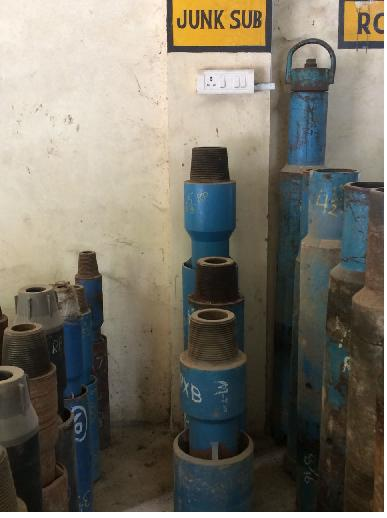
\includegraphics[scale=0.3]{images/junksub}
\centering 
\caption{A Picture of Junk sub}
\end{figure}


\item \textbf{Reverse Circulation Junk Basket:} The Reverse Circulation Junk
basket or RCJB is used to retrieve all types of small junk objects in
wellbore. By producing a circulating force with jet nozzles the junk
basket is capable of retrieving the most stubborn items in the hole
bottom such as bit rollers, bit bearings, tong dies, hand tools.The Assembly consists of top sub, bowl, junk catcher, value
assembly and shoe.The reverse circulation is made possible by hollow barrel.

\begin{figure}[h]
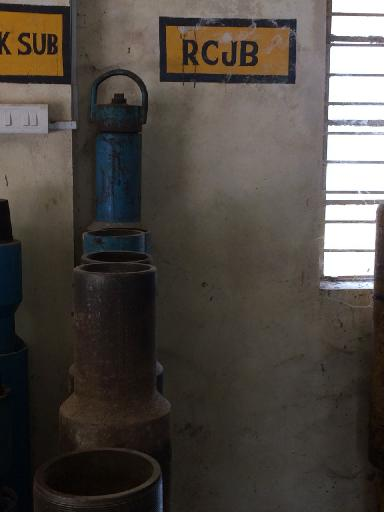
\includegraphics[scale=0.3]{images/RJCB}
\centering 
\caption{A Picture of Reverse Circulation Junk Basket}
\end{figure}


\item \textbf{Overshot:} Overshot is a positive engagement and disengageable tool.
Positive engagement means the overshot is capable of withstanding
even jarring impact (F.S. type). Disengageable means, it can be
disengaged from the fish at any position/depth.It is designed to catch smooth round tubular o/d fish.
The standard overshot is as the equivalent tool joint strength for screw in
connection, Excluding slim hole overshot. It can be disengaged
from fish on requirement basis.

\begin{figure}[t]
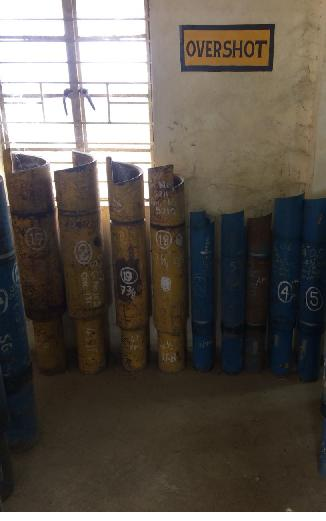
\includegraphics[scale=0.3]{images/overshot}
\centering 
\caption{A Picture of overshot}
\end{figure}

\item \textbf{Fishing Magnet:} It is used to retrieve undrillable material having
magnetic attraction. Small odd shaped items like bit rollers, dies, tong
pins etc. which cannot be retrieve by any outside or inside catching
tools. They can be run on wire line or drill string.


\begin{figure}[h]
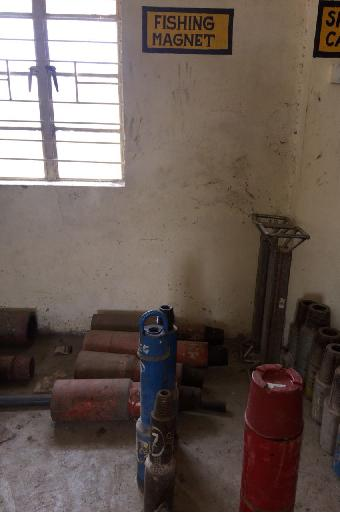
\includegraphics[scale=0.3]{images/fishing_magent}
\centering 
\caption{A Picture of Fishing Magnet}
\end{figure}


\item \textbf{Die Collar:} Rotary Die Collar are the simplest fishing tool available
for engaging a fish externally. This is not a positive engagement tool.
It consists of wickers which are non-fluted design if circulation isrequired below the stuck point. Fluted type design also available to
flush cutting while engaging fish.

\begin{figure}[t]
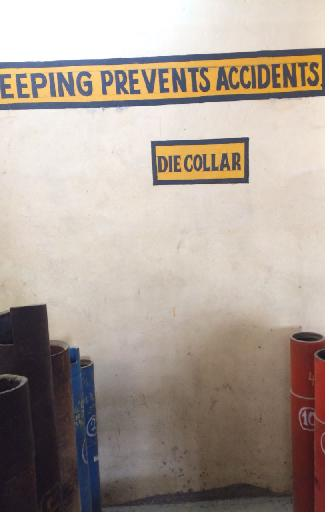
\includegraphics[scale=0.3]{images/Die_collar}
\centering 
\caption{A Picture of Die Collar}
\end{figure}

\end{itemize}



